\section{杠杆}\label{sec:7-1}

人们撬石头的时候,通常是象图 \ref{fig:7-1} 那样,把长棒的一端插到石头底下,再在长棒下面垫一块小石头,
然后用力压长棒的另一端,使长棒转动,将石头撬起。

\begin{figure}[htbp]
    \centering
    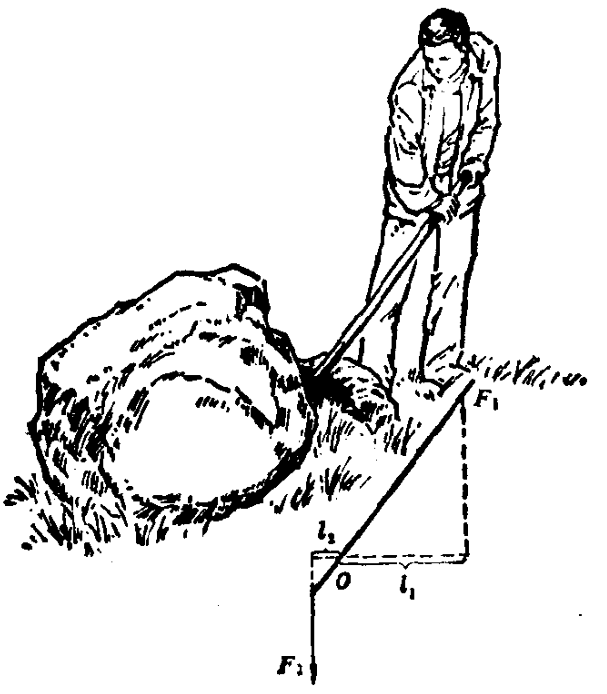
\includegraphics[width=0.4\textwidth]{../pic/czwl1-ch7-1}
    \caption{}\label{fig:7-1}
\end{figure}

\begin{figure}[htbp]
    \centering
    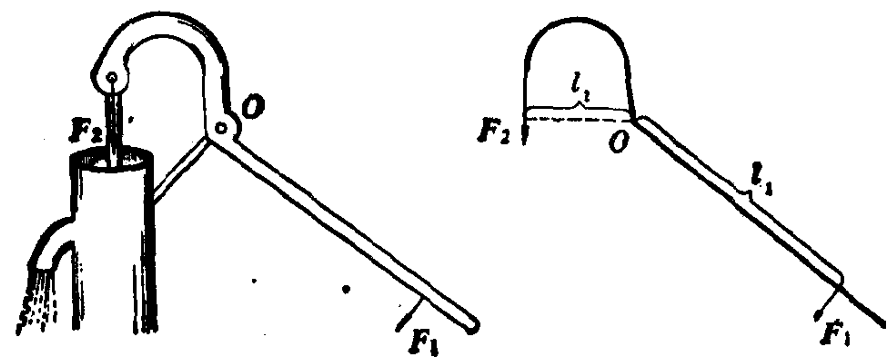
\includegraphics[width=0.6\textwidth]{../pic/czwl1-ch7-2}
    \caption{}\label{fig:7-2}
\end{figure}

一根硬棒,在力的作用下如果能绕着固定点转动,这根硬棒就叫做\textbf{杠杆}。

杠杆可以是直的,也可以是弯的,图 \ref{fig:7-2} 所示的抽水机的柄就是一根弯的杠杆。
用力压柄的一端,使柄绕着固定点 $O$ 转动,柄的另一端就克服活塞阻碍柄转动的力,把活塞提上来。

手作用在杠杆上使杠杆转动的力 $F_1$,叫做\textbf{动力}。
石头或活塞作用在杠杆上阻碍杠杆转动的力 $F_2$,叫做\textbf{阻力}。
杠杆绕着转动的固定点 $O$ 叫做\textbf{支点}。
从支点到动力的作用线\footnotemark 的垂直距离 $l_1$,叫做\textbf{动力臂}。
从支点到阻力的作用线的垂直距离 $l_2$,叫做\textbf{阻力臂}。

\footnotetext{通过力的作用点沿力的方向所引的直线,叫做力的作用线。}

从经验知道,撬石头的时候,需要加在杠杆上的动力 $F_1$ 的大小,不仅跟阻力 $F_2$ 的大小有关系,
还跟动力臂和阻力臂的长短有关系。动力臂越长,阻力臂越短,我们就越省力。
那么,动力、动力臂、阻力、阻力臂之间究竟存在什么样的关系呢?下面用实验来研究这个问题。

